\hyphenation{se-para-tion}
\hyphenation{theo-re-ti-cal}
\hyphenation{handed-ness}
\hyphenation{fo-llo-wing}
\hyphenation{ac-cor-ding}

\chapter{Theory}
\label{ch:theory}


In the previous chapter, we introduced the SM and discussed the particles and their interactions that are described by this theory. In this chapter we will start with the general mathematical formalism of the SM. Then, in the second part we will focus on the double Higgs boson physics described in Beyond the Standard Model (BSM) theories.

\section{Lagrangian formalism of the Standard Model}


\indent The SM uses Lagrangian mechanics as the mathematical approach to describe quantitatively the interactions of elementary particles and fields. 
The SM Lagrangian can be split into four main contributions \cite{Mozer:2016wzi}:
\begin{equation}\label{lagr_SM}
\Lagr_{SM} = \Lagr_{Yang-Mills} + \Lagr_{ferm} + \Lagr_{H} + \Lagr_{Yuk} 
\end{equation}

\noindent where

\begin{itemize}
\item $\Lagr_{Yang-Mills}$ represents gauge bosons and their \textcolor{black}{self-}interactions,
\item $\Lagr_{ferm}$ describes fermions and their interactions with the gauge bosons, 
\item $\Lagr_{H}$ characterises the Higgs boson, its self-interaction, and its interaction with the gauge bosons to give them mass, 
\item $\Lagr_{Yuk} $ gives details of fermions and their interactions with the Higgs boson, which, through the Yukawa mechanism, give mass to fermions.
\end{itemize}
 

The first term in the SM Lagrangian in full can be written as:
\beqn\label{lagr_Yang-Mills}
\Lagr_{Yang-Mills} = 	-\frac{1}{4}W^i_{\mu\nu}(x)W_i^{\mu\nu}(x) -\frac{1}{4}B_{\mu\nu}(x)B^{\mu\nu}(x) -\frac{1}{4}G^a_{\mu\nu}(x)G_a^{\mu\nu}(x)
\eeqn

\noindent where

\begin{align}
B_{\mu\nu}(x)   \equiv & \partial_\mu B_\nu -  \partial_\nu B_\mu \label{B_tensor} \\ 
W^i_{\mu\nu}(x) \equiv & \partial_\mu W^i_\nu(x) - \partial_\nu W^i_\mu(x) - g \varepsilon^{ijk}W^j_\mu W^k_\nu \label{W_tensor}\\
G^a_{\mu\nu}(x) \equiv & \partial_\mu G^a_\nu(x) - \partial_\nu G^a_\mu(x) - g_s f^{abc}G^b_\mu G^c_\nu \label{G_tensor}
\end{align}


\noindent with $\mu$ and $\nu$ indices running from 0 to 3, \textit{SU(2)} indexes $i,j,k = 1,2,3$, and \textit{SU(3)} indices given by $a,b,c = 1, ..., 8$. Terms $\partial_\mu$ and $\partial_\nu$ represent four-vector covariant derivatives. According to the Noether's theorem, each symmetry is intrinsically connected to a conservation law \cite{Sardanashvily:2143630}. The invariance of the Lagrangian under certain transformations or, in other words, how the fields in the Lagrangian ($\Lagr_{Yang-Mills} $ in this case) are related to their corresponding underlying symmetries, is explained in the following way: 

\begin{itemize}
\item $B_{\mu\nu}$ corresponds to \textit{$U(1)_Y$} symmetry of the weak hypercharge $Y_k$ with \textit{U(1)} being a unitary one-by-one matrix (a scalar), 
\item $W^i_{\mu\nu}$ corresponds to \textit{$SU(2)_I$} symmetry of the weak isospin $I^i_{w}$. Another common representation is \textit{$SU(2)_L$}, since only left-handed SM fermions are transformed under this symmetry. \textit{$SU(2)_L$} is a unitary two-by-two matrix with the determinant equal to one. 
\item $G^a_{\mu\nu}$ corresponds to \textit{$SU(3)_c$} symmetry of the QCD color charge with \textit{$SU(3)_c$} being a unitary three-by-three matrix with the determinant equal to one.
\end{itemize}

\noindent The "B" field is a kinematic term, "W" and "G" terms describe interactions among the gauge bosons, $g$ and $\varepsilon$ are \textit{$SU(2)_L$} coupling and structure constants, $g_s$ and $f$ are coupling and structure constants for \textit{$SU(3)_c$}.


The second term in the SM Lagrangian is: 
\beqn\label{lagr_ferm}
\Lagr_{ferm}= i \bar{\Psi}_L \slashed{D} \Psi_L  + i \bar{\psi}_{l_{R}}  \slashed{D} \psi_{l_{R}} +
i \bar{\Psi}_Q \slashed{D} \Psi_Q  + i \bar{\psi}_{u_{R}}  \slashed{D} \psi_{u_{R}} +
 i \bar{\psi}_{d_{R}}  \slashed{D} \psi_{d_{R}}
\eeqn

\noindent Notice, that the mass terms are still absent. In Eq. \ref{lagr_ferm}, $\Psi$ represents a doublet of a charged lepton and a corresponding neutral lepton within the same lepton family of \textit{$SU(2)_L$}. The subindex Q is reserved for a family of quarks, and $\psi_R$ describes a right-handed leptonic singlet.  Gauge boson interactions are present due to the derivative term:
\begin{align}\label{cov_der2}
D_\mu = \partial_\mu + ig I_w^i W_\mu^i+ ig' Y_w B_\mu + ig_s T_c^a G_\mu^a
\end{align}

\noindent Physical fields in this notation are represented by a linear combination of W and B fields:
\begin{align}\label{neutral_fields}
A_\mu = &  B_\mu \cos\theta_W + W^3_\mu \sin\theta_W \\ 
Z_\mu = & -B_\mu \sin\theta_W + W^3_\mu \cos\theta_W \nonumber 
\end{align}
\noindent where $\theta_W$ is known as the \ti{Weinberg angle} \cite{Weinberg:799984}.

With the first two terms of the SM Lagrangian --  $\Lagr_{Yang-Mills}$ and $\Lagr_{ferm}$ -- one obtains a valid theory of fermions and bosons; however, these particles are massless in this theory \cite{Wolf:2015kua}, which evidently contradicts reality. However, one cannot simply add mass terms by hand since that would break the Lagrangian gauge invariance. To solve this issue and to ensure that weak bosons are massive, one has to follow a more complex procedure: introduce a Higgs field and an SSB procedure (see section \ref{sec:BEH}). During the SSB procedure, the $SU(2)_L \times U(1)_Y$ symmetry needs to be broken to have massive SM particles. The Higgs mechanism enters the SM Lagrangian through the corresponding Higgs Lagrangian term given by 
\beqn\label{lagr_higgs}
\Lagr_H=(D_\mu\Phi)^\dagger(D^\mu\Phi) - V(\Phi) , \qquad V(\Phi)= - \mu^2(\Phi^\dagger\Phi) + \frac{\lambda}{4}(\Phi^\dagger\Phi)^2
\eeqn

\noindent where

\beqn\label{vev}
\Phi = \binom{\phi^+}{\phi^0 = (v+H + i\chi)/ \sqrt{2}} \quad \text{with} \quad v = 2 \sqrt{\frac{\mu^2}{\lambda}}
\eeqn

\noindent and $\mu$ and $\lambda$ are parameters of the Higgs potential. The Higgs field vacuum expectation value ($vev$) $v$, after the SSB, can be expressed in terms of $\mu$ and $\lambda$. The Higgs potential before and after the SSB is shown in Fig. \ref{hp2d}. The importance of the $\Lagr_H$ in the SM Lagrangian is crucial: after rearranging terms (full derivation is available at \cite{Halzen:100339, Zee_qft}), the bosons finally have masses given by:

\beqn\label{boson_masses}
M_W = \frac{gv}{2}, \quad  M_Z = \frac{M_W}{\cos{\theta_W}}, \quad M_H = \sqrt{2\mu^2}
\eeqn



 
The final contribution to the SM Lagrangian is the Yukawa term, with Yukawa Lagrangian given by:
\beqn\label{lagr_Yuk}
\Lagr_{Yuk}=  - i \bar{\Psi}_{L}  G_l  \psi_{l_{R}} \Phi
- i \bar{\Psi}_{Q}  G_u  \psi_{u_{R}} \tilde{\Phi}
- i \bar{\Psi}_{Q}  G_d \psi_{d_{R}} \Phi + h.c.
\eeqn

\noindent where $\tilde{\Phi} = i \sigma^2 \Phi^*$. The $3 \times 3$ matrices G contain fermion masses, which are free parameters in the SM and have to be determined experimentally. These matrices  describe  the  so-called Yukawa $y_f$ couplings between the single Higgs doublet $\varphi$ and the fermions. In the case of leptons, matrices G can be diagonalised to provide mass eigenstates of definite generation. Using the mass eigenstates, the strength of the coupling of a fermion $y_f$ to a Higgs boson is given by $y_f = m_f /\textit{vev}$, where $m_f$ is the mass of a fermion and \textit{vev} is set by $\mu$ and $\lambda$ parameters, see Eq. \ref{vev}. On contrast, W and Z boson masses are predicted by the SM and are directly related to the weak couplings and the Higgs field parameters, see Eq. \ref{boson_masses}. 
%The mass of each fermion is proportional to the Yukawa coupling ($y_f$ or $\lambda_f$) of the corresponding fermion to the Higgs boson, as shown in Fig. \ref{coupling_ff}.


The Higgs boson mass is proportional to the $\mu$ parameter. In 2012, using precise single Higgs boson mass measurements from both ATLAS and CMS experiments, the value of $\mu$ was determined. Additionally, many physics analyses at CERN have been targeting the measurement of the $\lambda$ parameter, because it is related to the shape of Higgs potential. The simplest potential characterized by $\mu$ and $\lambda$ parameters, sufficient to obtain the SSB phenomenon and give mass to the SM particles, is the so-called "Mexican hat" Higgs potential. This name reflects the fact that the shape of the potential after SSB resembles the Mexican hat, see Fig. \ref{hp2d}. However, the real shape of the Higgs potential may be more complex or different from the Mexican Hat, thus, direct precise determination of the $\mu$ and $\lambda$ parameters is a sensitive tool to test the limitations of the SM and may open doors to the BSM effects. The simplest interaction suitable for probing the higher order terms of the Higgs potential directly is the one where two Higgs bosons (HH) are present. All this makes HH physics, the topic of this thesis, one of the main goals for the future High Luminosity LHC (HL-LHC) that will start operations in 2026. 

\begin{figure}[H]
\centering
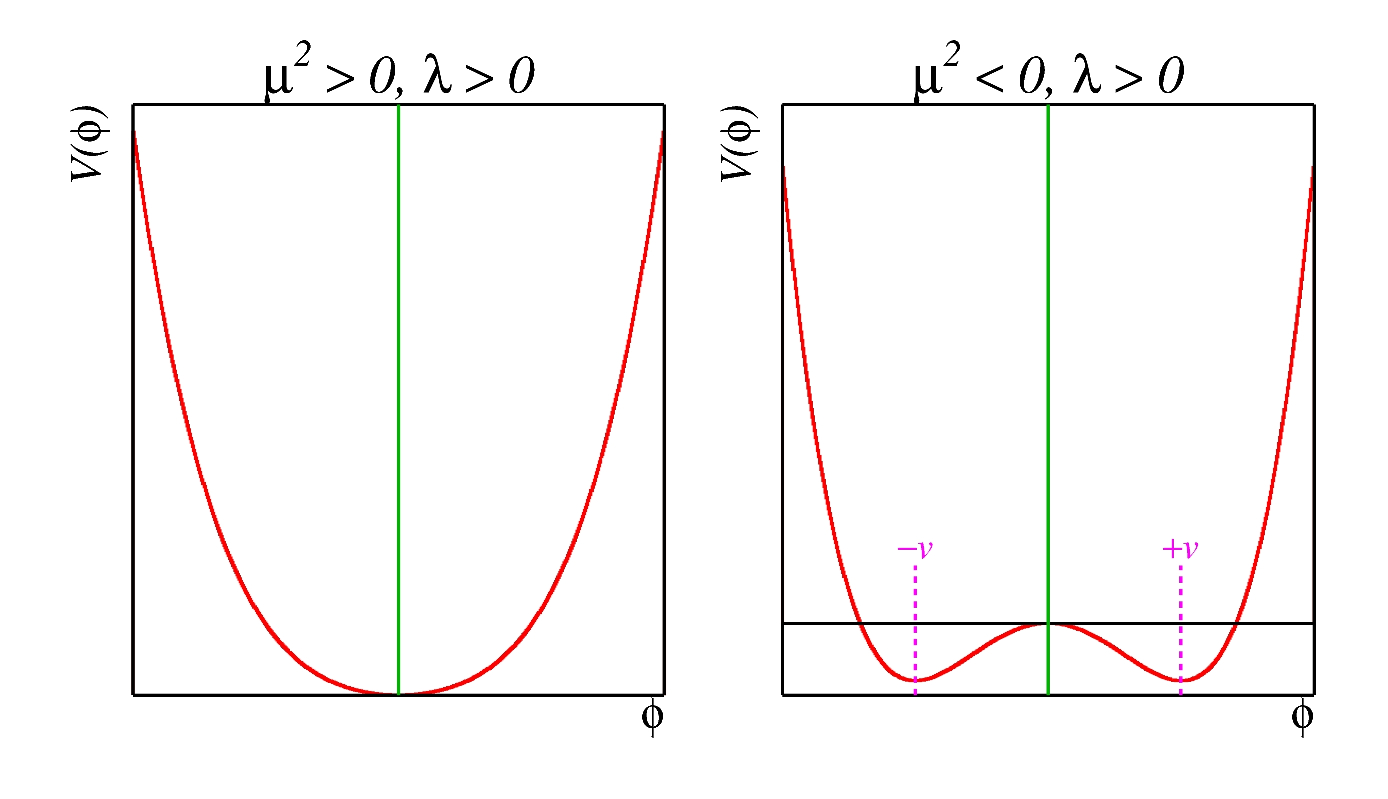
\includegraphics[width=0.7\textwidth]{hp2d}\\
\hspace{1cm} 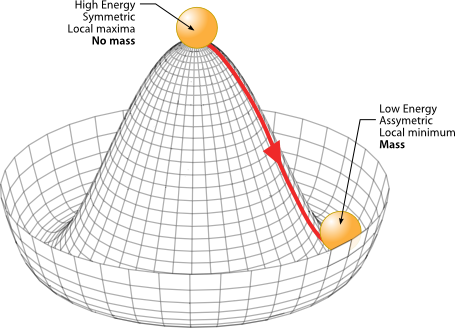
\includegraphics[width=0.44\textwidth]{higgs-hat}
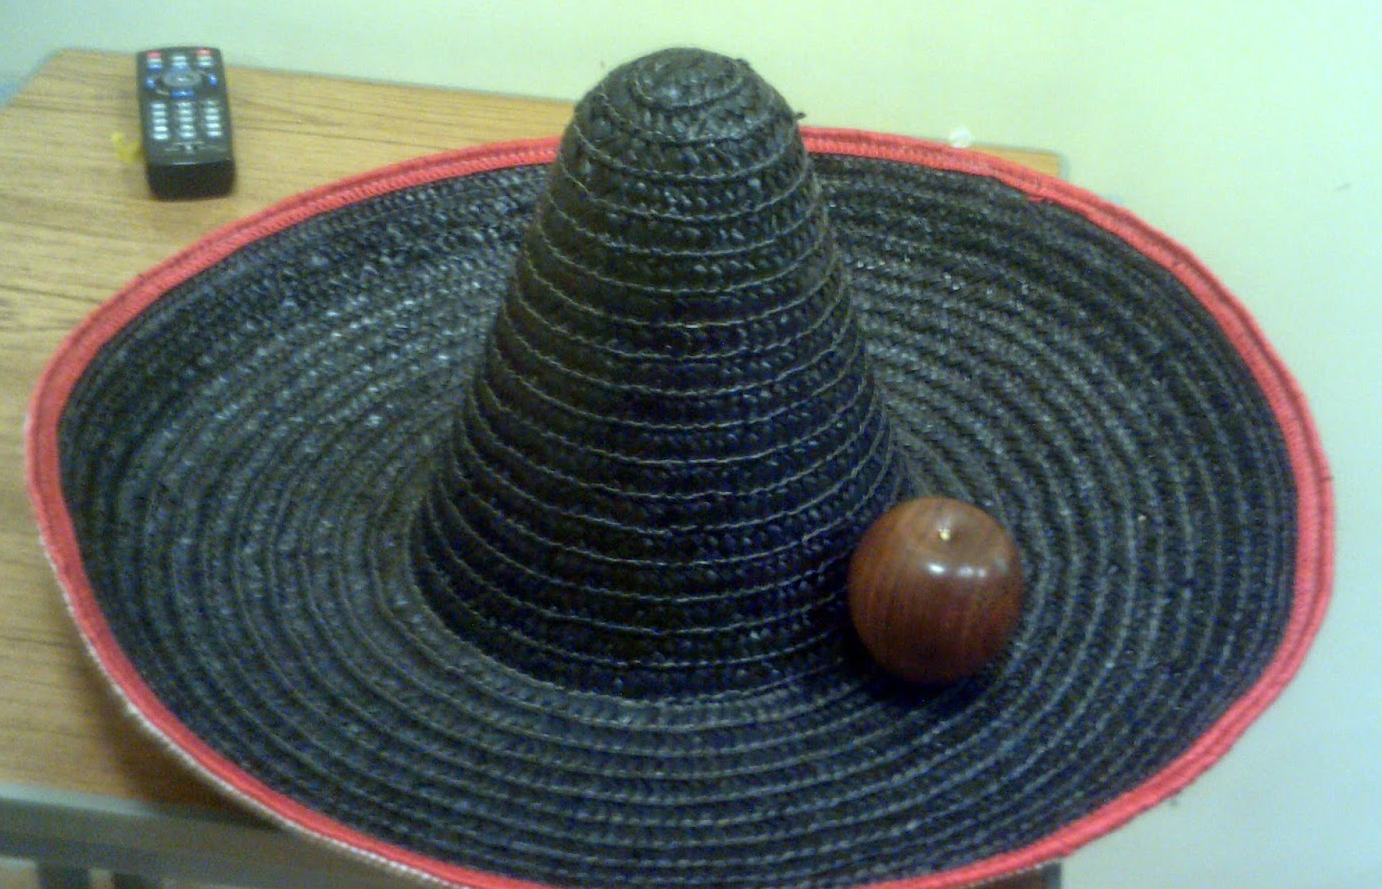
\includegraphics[width=0.4\textwidth]{mexican2}\\
\caption[SSB Potential form]{Top: Shape of the Higgs potential before and after the SSB that is determined at the leading orders by $\mu$ and $\lambda$ parameters \cite{MonroyMontanez:2639240}. Bottom Left: Schematic drawing of the Higgs potential (after the SSB) that resembles a Mexican hat. Bottom Right: A real Mexican hat.}
\label{hp2d}
\end{figure}


\section{Double Higgs in Beyond the Standard Model Theories}

%\textcolor{red}{IN THE INTRO??}
While the mass parameter $\mu$ has been measured fairly accurately, $\lambda$ parameter requires even HL-LHC to run for many years to get enough statistics since HH processes are rare and are of almost three orders of magnitude lower rate than the single Higgs boson production. Technically, the amount of the HL-LHC data is not enough to reach the sensitivity of the SM for HH processes. However, several BSM models predict resonant HH production to which the current LHC data could be sensitive. In these theories, HH is produced through a decay of a heavy resonance, which is not a part of the SM; thus, if such processes are found, a new chapter in HEP will be opened. In this thesis we focus on the resonant production of the HH system, which further decays to leptons and quarks. With the available CMS data, resonant HH analyses are starting to approach the needed sensitivity to many BSM models. 

BSM theories such as \cite{Huang:2017nnw, Dolan:2012ac, Kanemura:2016tan, Sirunyan:2018iwt, Randall:1999ee, Oliveira:2014kla} predict a resonant production of double Higgs boson events through a heavy resonance of a narrow width ($\sim O(1-10)$ GeV) \cite{Sirunyan:2018iwt}. Since the width parameter is proportional to the mass of the particle and its coupling to the Higgs boson, the values of the width larger than the $1-10$ GeV  range would correspond to BSM particles too heavy to be produced at the LHC. Additionally, from the perspective of the experimental physicist, the ``bump hunt'' of a narrow width particle is the well-established technique that led to discoveries of many particles. 


In this dissertation data is compared to predictions from the Warped Extra Dimensions theory (WED) \cite{Oliveira:2014kla}. WED theory addresses the hierarchy problem by adding an additional fifth dimension to the conception of 4-dimensional (4D) space-time. In the framework introduced by Randall and Sundrum (RS) \cite{Randall:1999ee}, 4D space is an Effective Field Theory (EFT) approximation of the higher dimensional space. The extra dimension exists between the gravity (Planck) and weak (TeV) flat 4D branes (see Fig. \ref{branes}) and is called the "bulk". In the bulk, the strength of the gravitational interaction is not uniform. It depends on the coordinate in the 5th dimension and is characterised by the exponentially decaying function.




\begin{figure}[H]
\centering
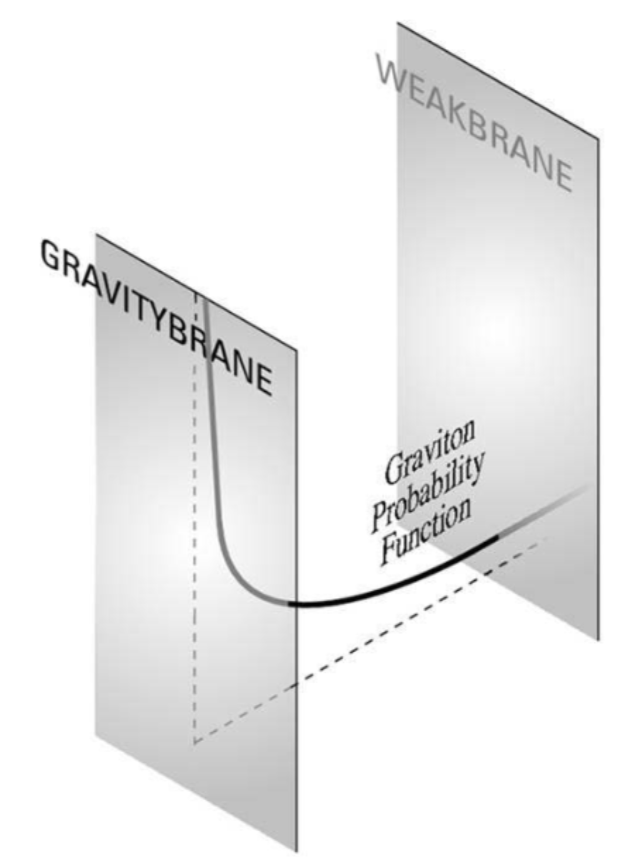
\includegraphics[width=0.4\textwidth]{branes.png}
\caption[RS branes]{5D space in the RS model \cite{Xanda}.}
\label{branes}
\end{figure}




The free parameters of the RS model are the brane separation factor $k$ and the size of the compactified dimension $r_c$. Another name for the brane separation factor is the curvature factor. This factor is given by $k \approx \sqrt{ \frac{\Lambda}{M^2_5}  }$, where $\Lambda$ is the ultraviolet cutoff of the theory and $M_5$ is the 5D Planck mass. %The radius of the extra dimension $r_c$ is proportional to the parameter $1/k$ and the logarithm of $1/vev$. 
The mass hierarchy of the SM particles between the Planck scale and the electroweak scale can be reproduced when free parameters $k$ and $r_c$ satisfy $k \cdot r_c \approx 11$. In this case, the RS model matches the observations: the Higgs boson being closer (in the geometric sense in the fifth dimenstion) to the TeV brane and light fermions being located near the Planck brane, see Fig. \ref{branes}.

In the RS model under study, two new particles appear: a graviton and a radion. When the bulk is compactified, the WED theory predicts the existence of the Kaluza-Klein (KK) \cite{Uzawa:1999pg} excitations of the gravitational field, with the zero-th KK mode being a graviton, the mediator of the gravitational force. The graviton (spin 2) is the first WED particle predicted by the RS model. The graviton can propagate freely in the full higher-dimensional space of the 5D bulk. The other RS particle is a radion (spin 0). Its existence is required to stabilise the size of the extra dimension. The WED space necessarily behaves in a quantum way, and, therefore, its size or length is subject to quantum fluctuations. The fluctuations of the length are parametrised by the radion, which is very similar to how the fluctuations of the EM field are parametrized by the photon. Goldberger and Wise \cite{Goldberger:1999uk} wrote down a potential for the radion and showed how \textit{vev} of the radion sets the length of the extra dimension to its desired value. This is the mechanism for stabilizing the WED length. Without this procedure the radion would be massless and would mediate an infinite-range interaction, which is in conflict with cosmological observations. 


Since LHC had provided us with no evidence of the SM particles interacting with the RS particles, the RS model considered in this thesis hypothesizes that SM particles are confined to branes. Another explanation of the lack of evidence of the RS particles at the LHC could be due to the fact that RS particles are too massive to be produced at the current LHC energies, but this argument is not addressed in this dissertation. 


The theoretical arguments put forward by the authors \cite{Davoudiasl:1999jd} suggest the RS parameters $k$ and $\bar{M}_{Pl}$ to be constrained by the following range of values: $0.01 \leq k / \bar{M}_{Pl} \leq 1$, where the parameter $k$ is of the order of the Planck scale and $\bar{M}_{Pl} = \sqrt{\frac{M^3_5}{k} \cdot (1 - e^{-2\pi k r_c} ) }$ is a reduced 4D $M_{Pl}$. Considered in this measurement, the graviton and radion are RS particles with a KK state mass of the order of TeV \cite{Oliveira:2014kla}. 

With a part of the KK 5D wave function, often called a profile, expressed as $f^{(n)}_X(\phi)$, where n refers to the n$^{th}$ KK mode, the graviton can be decomposed as $\sum_{n=0}^{\infty} h^{(n)}_{\mu\nu}(x_\mu) \cdot f^{(n)}_X(\phi)$. Its zero-th mode corresponds to the massless graviton and the first mode corresponds to the lightest KK graviton (later graviton) which has the mass of the O(TeV). The profiles for all the matter fields are described by a combination of Bessel and exponential functions \cite{Traczyk:2002jh, Goldberger:1999wh,Raychaudhuri:2126967}. The Lagrangian describing the interaction of the graviton with the SM fields is given then by 

\beqn\label{lagr_graviton}
\Lagr_{graviton}=  - \frac{x_1\tilde{k}}{m_G} h^{\mu\nu(1)} \times d_i T^{(i)}_{\mu\nu},  
\eeqn
where $x_1$ = 3.83 is the first zero of the Bessel function for a given profile, $\tilde{k}  = k / \bar{M}_{Pl}$, $h^{\mu\nu}$ is a tensor describing the first KK graviton field, $m_G$ is the mass of the graviton of the order of TeV, $d_i$ is an integral of the profiles of the SM fields and KK graviton, and  $T^{(i)}_{\mu\nu}$ is a 4D canonical energy-momentum tensor \cite{Forger:2003ut} for any SM field $i$. A free parameter $\tilde{k}$ varies from 0.01 to 1 when $m_{G}$ is varied from 100 to 1500 GeV. 

For the radion, the Lagrandian is given by:
\beqn\label{lagr_radion}
\Lagr_{radion}=  - \frac{r}{\Lambda_R} \times a_i T^{\mu (i)}_{\mu},  
\eeqn
where $r$ is a 5D radion field, $\Lambda_R$ is the scale parameter proportional to $k \cdot \sqrt{ ( \frac{M_5}{k} )^3}$, and $a_i$ is the coupling of the radion to the SM field $i$. In the studied RS model the profiles of the graviton and radion arise naturally as being localised at the TeV brane for the coupling of a radion and a graviton to the massive SM fields to have the value of the order of one \cite{WED}. 


In the SM, HH production is dominated by two processes, which are shown using Feynman diagram representation in Fig.\ref{SM_HH}: the "box" and the "triangle" diagrams. They interfere destructively and the total cross section is thus lowered. The total cross section made of box and triangle contributions is denoted as the ``SM'' and is shown in black color in Fig. \ref{hh_comparison} on the right. Additionally, this figure includes a BSM contribution - a non-linear (``nl'') term $t\bar{t}HH$ that vanishes in SM, but may be present in BSM \cite{Contino:2012xk}. The results shown in Fig. \ref{hh_comparison} right, have been produced by theorists \cite{Chen:2014xra} for 100 TeV collider. However, the distributions of the double Higgs mass as well as amplitudes remain to a high degree unchanged between 13-14 and 100 TeV (see Fig. \ref{hh_comparison} on the left) - therefore, one assumes that amplitudes would look similarly for 13 TeV. 

\begin{figure}[H]
  \centering
    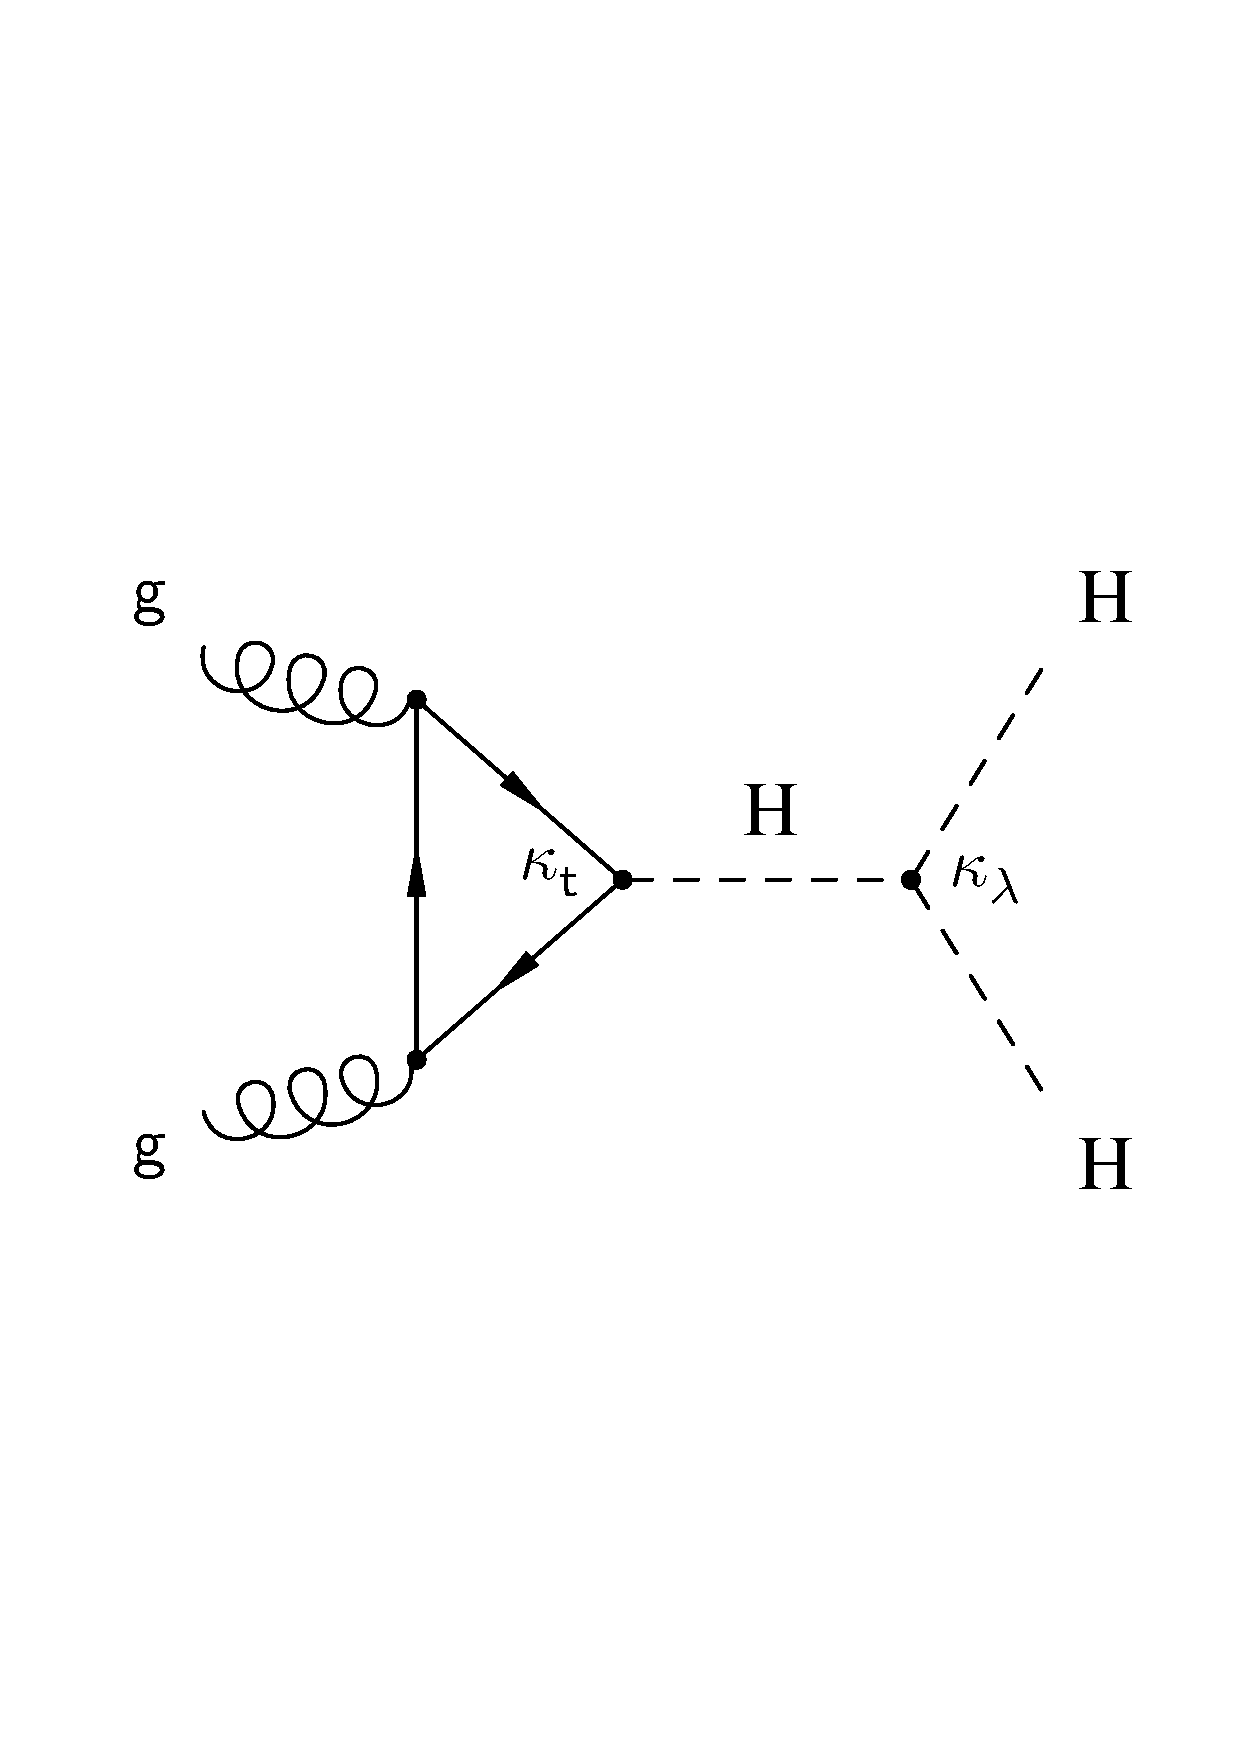
\includegraphics[width=0.49\textwidth]{hh_tri}
     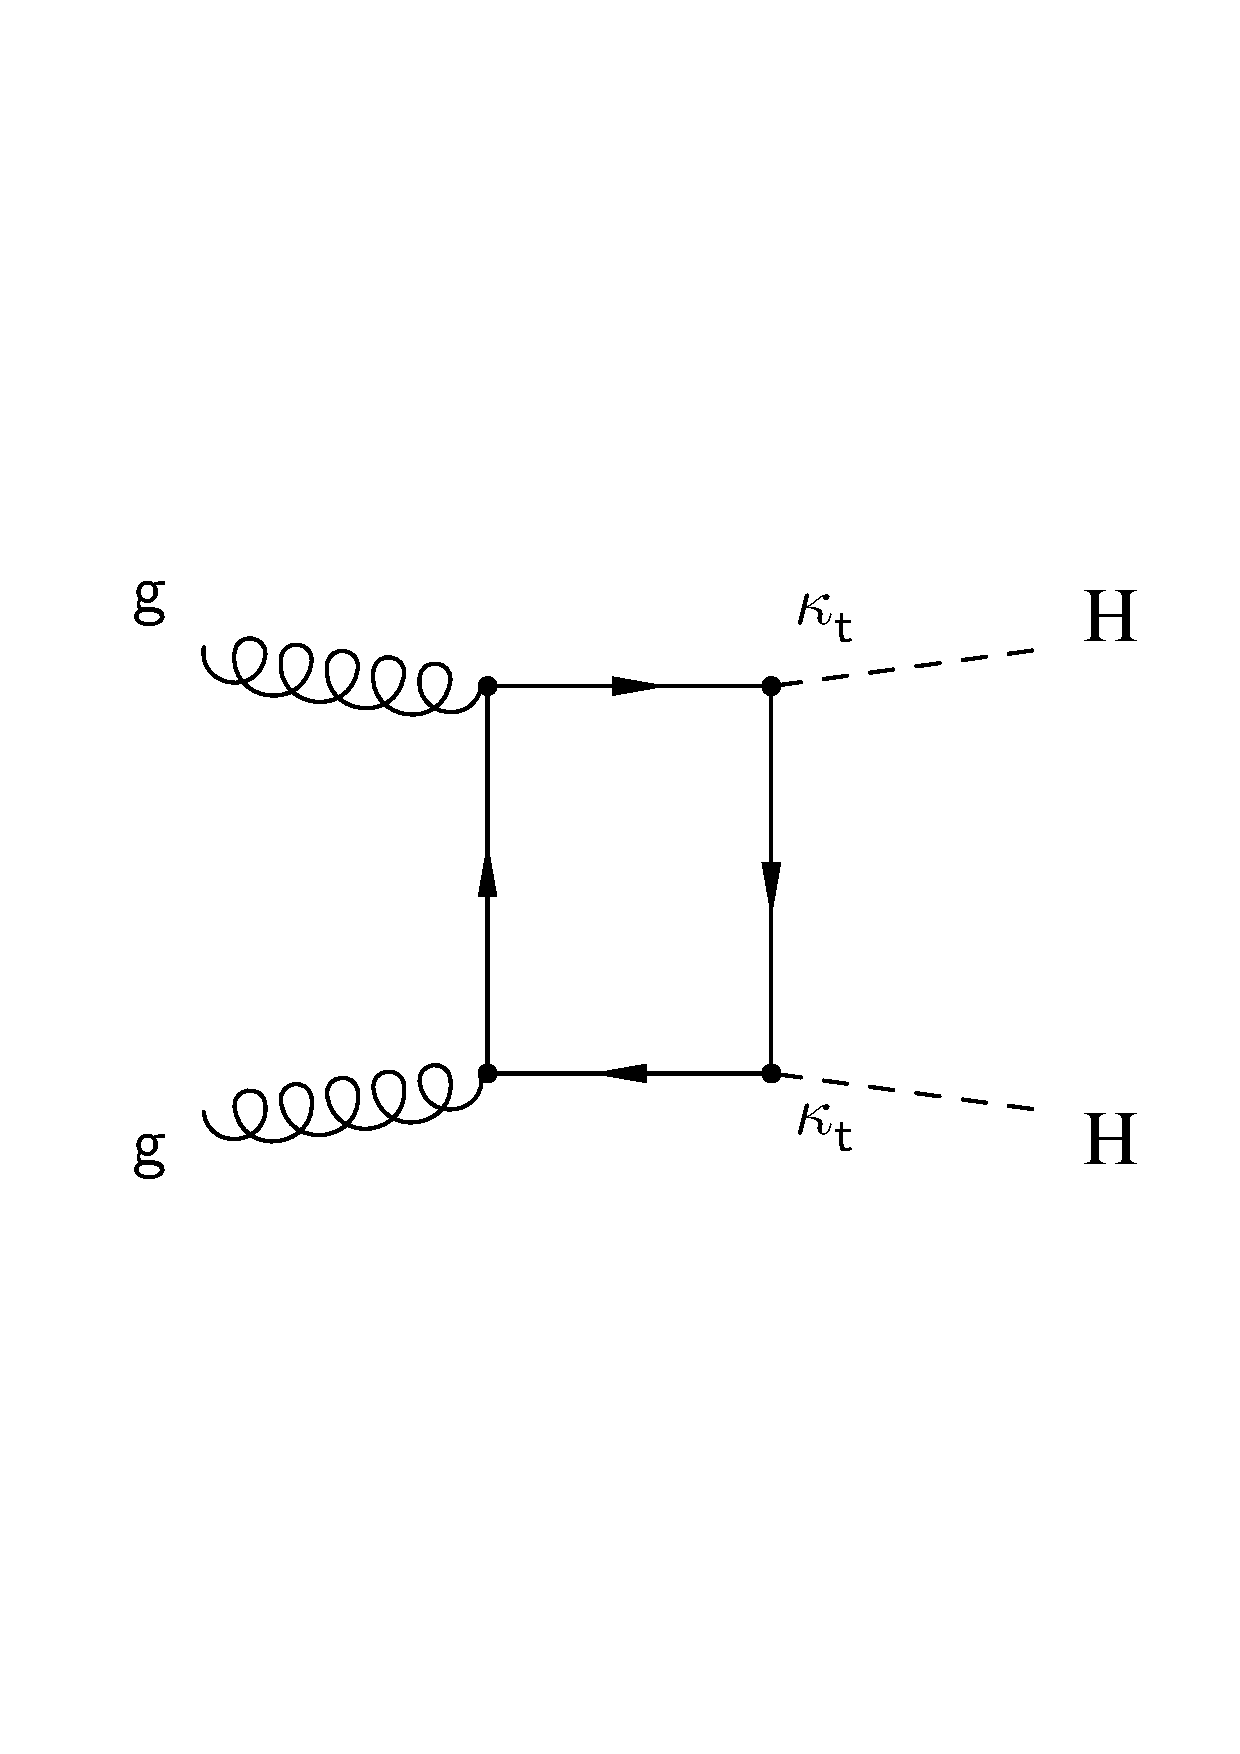
\includegraphics[width=0.44\textwidth]{hh_box_2}
    \caption[SM double Higgs boson production]{SM double Higgs boson production. Left: the triangle diagram with the virtual top quark loop. Right: the box diagram which dominates the overall HH production rate.}
    \label{SM_HH}
\end{figure}

The box diagram dominates the double Higgs boson production and peaks near 400 GeV of the di-Higgs mass \cite{Chen:2014xra}. Even though the Fig. \ref{hh_comparison} on the right illustrates the SM double Higgs production, which is a non-resonant process, the amplitudes are not flat. Two factors contribute: an amplitude decreases with the COM and, at the same time, the kinematic turn on of the production of the di-Higgs system is always present. 



\begin{figure}[H]
  \centering 
    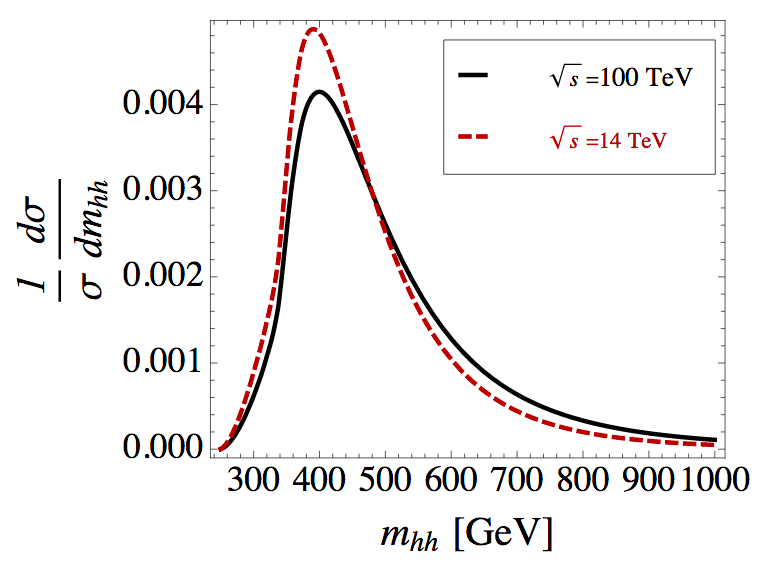
\includegraphics[width=0.49\textwidth]{hh_14_100_comparison}
    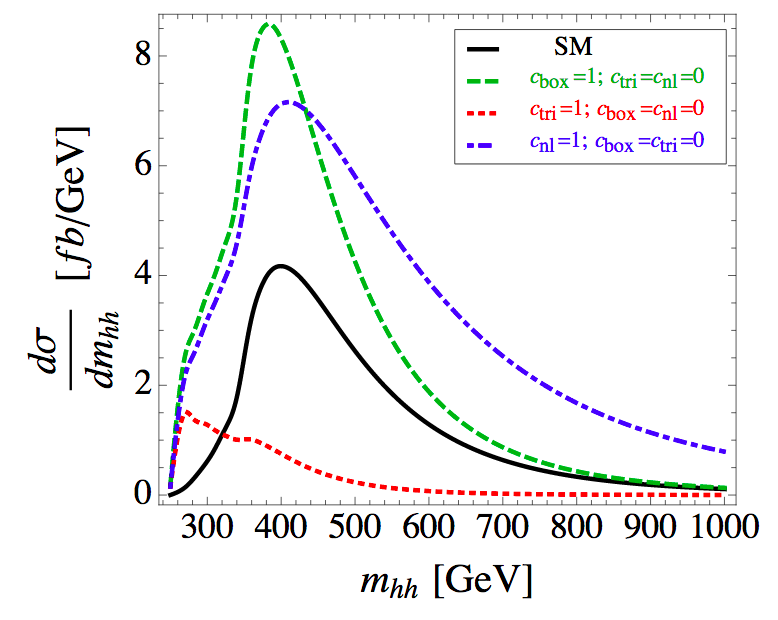
\includegraphics[width=0.49\textwidth]{hh_sm_comparison}
    \caption[Double Higgs mass distribution and the total cross-section]{Left: comparison of the double Higgs boson mass distribution in the SM at the LO at 14 and 100 TeV center-of-mass energy. Right: the total SM HH cross section and the individual contributions \cite{Contino:2012xk}. Green refers to the SM box production, red refers to the SM triangle production, and blue refers to BSM non-linear $t\bar{t}HH$ production, not included in the total SM production in black \cite{Chen:2014xra}. }
    \label{hh_comparison}
\end{figure}




In this measurement, the gravitons and radions in the search are expected to be produced by a BSM "contact interaction" Feynman diagram allowed by the WED scenario. This process is shown in Fig. \ref{HH_signature}.  A graviton and a radion decays to a pair of Higgs bosons are thoroughly studied theoretically \cite{Chen:2014xra, HHXsec, Contino:2012xk}. Experimental results produced by this measurement are compared to the theoretical predictions calculated for the WED model with the standard benchmark parameters $\tilde{k}=0.1$ and $\Lambda_R = 3 $ TeV \cite{Wertz:2632195, Cadamuro:2292733}. These reproduce SM observations and allow the production of the RS particles that can be observed at the LHC. 





\begin{figure}[H]
  \centering
    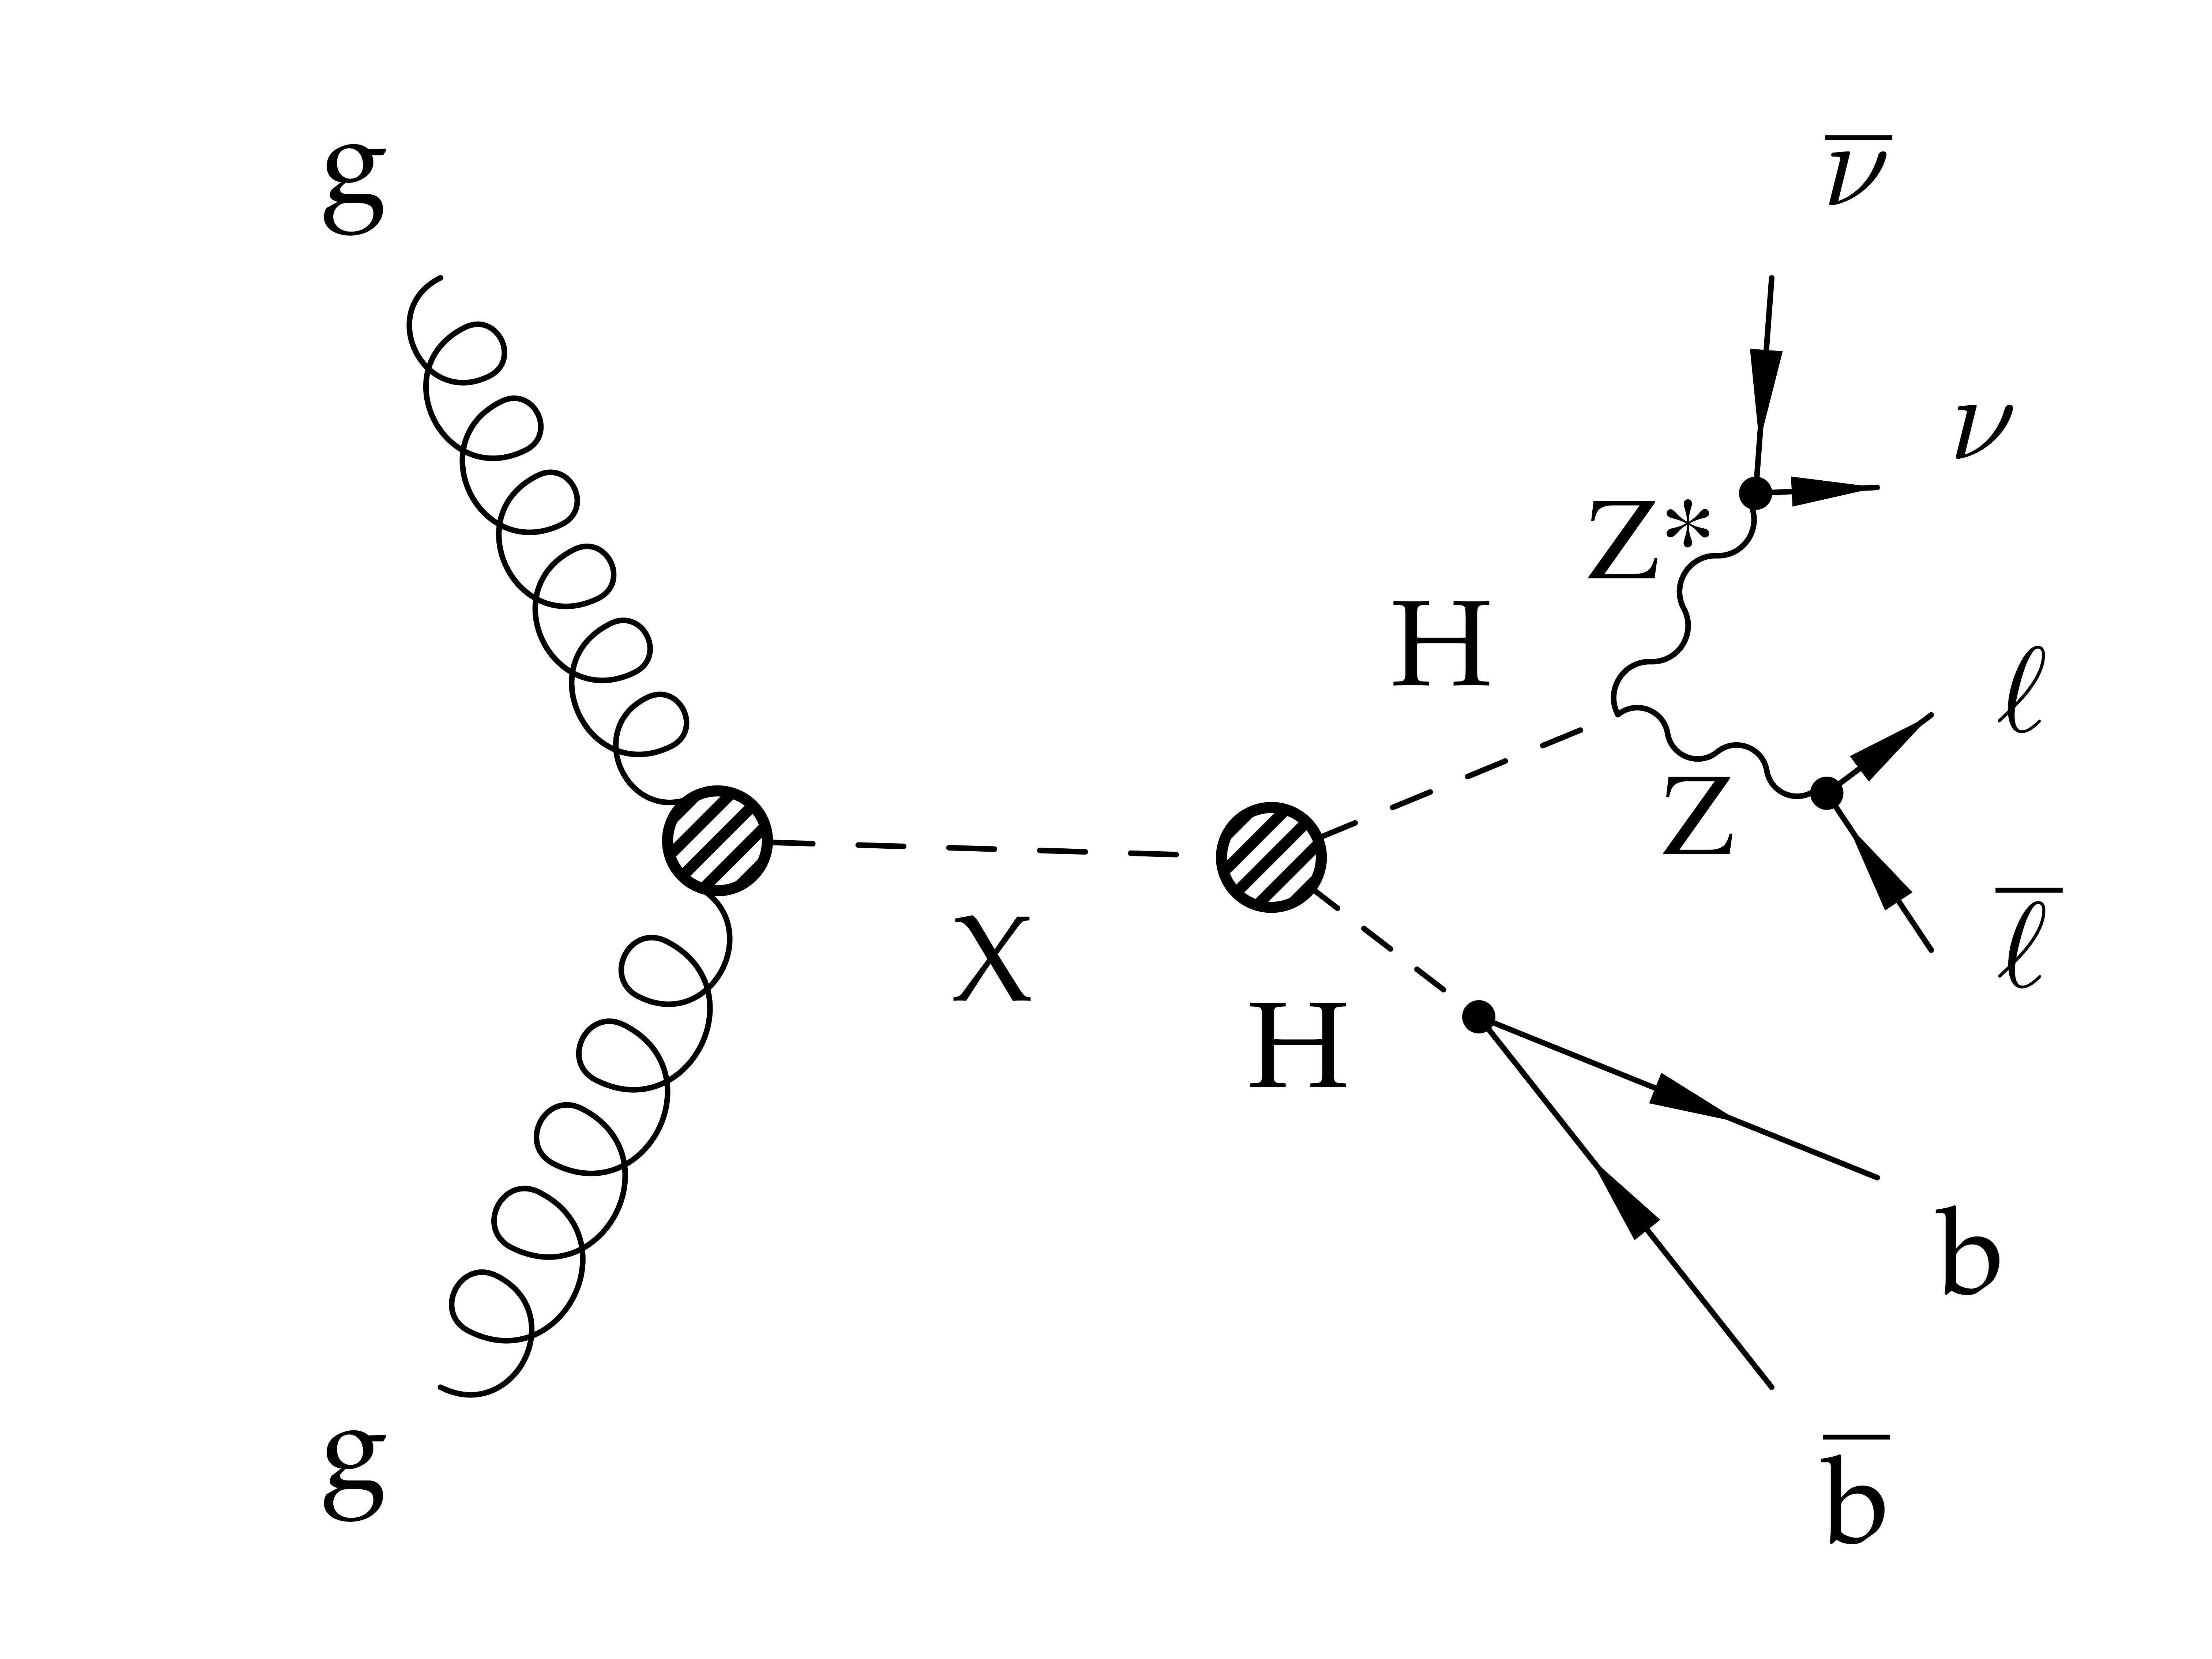
\includegraphics[width=0.50\textwidth]{HH_signature.png}
    \caption{BSM Resonant double Higgs decay in the 2 b, 2 lepton, and 2 neutrino final state. X denotes either graviton or radion particles. }
    \label{HH_signature}
\end{figure}




This thesis separately addresses both resonant graviton and radion decays into two SM Higgs bosons with the subsequent decays of one Higgs boson to a pair of b quarks, and the other Higgs boson to W or Z boson pairs. We select only leptonic W bosons decays. For Z boson decays, the chosen signature is characterised by the on-shell Z boson decaying into a pair of charged leptons and the off-shell Z boson decaying to neutrinos (see Fig. \ref{HH_signature}). The final state that this thesis focuses on consists of two b quarks, two charged leptons, and two neutrinos. Decays of the double Higgs system to this signature are observed on average in $2.8 \%$ of all di-Higgs decays. 


To finish this chapter, it is instructive to show all the decay channels of the double Higgs system to the SM particles, which are summarised in the Fig. \ref{BR}. Both the horizontal and the vertical axes show decays of a single Higgs boson to two SM particles. In this representation, each square on the plot specifies a branching fraction of one of the double Higgs boson decays, with the probability of the decay given by the color field map on the right axis. Our signature corresponds to 4 $\%$ of all $bbZZ$ decays, which are denoted on the map by the photo of the main $bbZZ$ analyser. 

\begin{figure}[H]
  \centering
    \includegraphics[width=0.50\textwidth]{BR2}
    \caption[Double Higgs decay channels]{Double Higgs decay channels. The SM branching fractions are represented by the color palette. In this measurement $bbZZ$ decays are analysed, which are denoted on the map by the photo of the main $bbZZ$ analyser.}
    \label{BR}
\end{figure}



